\documentclass{standalone}
\usepackage{varwidth}
\usepackage{sheets}
\usepackage{textcomp}

\newcommand*\cellEntryB[3]{\selecCell{#1}{#2}\celtxt[l,color=red]{#1}{#2}{#3}}

\begin{document}
\begin{varwidth}{\linewidth}
\centering

\begin{tikzpicture}
\tableur[2]{A,B,C,D}
\celtxt[r]{A}{1}{1}
\celtxt[r]{B}{1}{2}
\celtxt[r]{A}{2}{10}
\cellEntry{C}{1}{=A\textdollar 1}
\end{tikzpicture} 

$\downarrow$ Paste \texttt{C1} contents to \texttt{C2} and \texttt{D1}.

\begin{tikzpicture}
\tableur[2]{A,B,C,D}
\celtxt[r]{A}{1}{1}
\celtxt[r]{B}{1}{2}
\celtxt[r]{A}{2}{10}
\celtxt[r]{C}{1}{1}
\celtxt[r]{D}{1}{2}
\celtxt[r]{C}{2}{1}
\end{tikzpicture} 

\end{varwidth}
\end{document}
